\section{Results and discussion}
We will now first take a look at the case of two electrons in a potential with different oscillator energies. In order to do so, we preform a Variational Monte Carlo simluation and use the Metropolis algorithm explained in section~\ref{sec:metropolis} to find the energy of the ground state. Therefore we use numerical derivation. We will later introduce analytical calculations based on closed-form expressions as well (section~\ref{sec:analytical}). Besides, we put emphasis on the correlations introduced by the Jastro factor by computing the kinetic and potential energy of the ground state for different osciallator frequencies.\\
In addition we introduce importance sampling and analyse the dependency of the results to the time step $\delta t$.\\
\subsection{Two electron case}
Since it is the easiest case, we first look at two electrons in a quantum dot interacting with each other. According to \cite{taut} the corresponding energy is at $E = 3~\mathrm{a.u.}$ (atomic units).\\
Concerning the simulation we start by considering a wide range of $\alpha \in[0.7,1.3]$ and $\beta \in[0.2,0.6]$ first and preform a more precise simulation afterwards. The goal is to find the variational parameters $\alpha$ and $\beta$, where the energy is at its minimum. After the first simulation we notice, that the minimum must be somewhere around $\alpha \in[0.9,1.1]$ and $\beta \in[0.35,0.45]$. This is why we preform a somulation with these boundaries and use 3 000 000 Metropolis cycles to get an accurate result. In figure~\ref{fig:2electron} the energy is plotted depending on both variational parameters $\alpha$ and $\beta$. The 3D-plot results in a bended plane ressembling to a valley. For increasing $\alpha$ the corresponding $\beta$ at minimal energy is decreasing. The minimum energy calculated is 
\begin{align}
E &= 3.0003~\mathrm{a.u.}
\intertext{at}
\alpha &= 0.9867,\\
\beta &= 0.4033.
\end{align}
As mentioned before we were expecting the energy to be at $E=3~\mathrm{a.u.}$, so the calculated value matches the expected one very well.\\
To get a better understanding of the influence the parameters have on the calculated energy figure~\ref{fig:2electronalpha} shows the energy's $\alpha$-dependency for different $\beta$. Consistent with figure~\ref{fig:2electron} this figure shows, that the $\beta$ is shifted depending on $\alpha$ and that $\alpha$ has a larger influence on the energy. The errors plotted in figure~\ref{fig:2electronalpha} are almost invisible, since they are very small compared to the energy fluctuations at varying $\alpha$ and $\beta$. There are not many cases, where the error is significantly high, so we consider our results to be of sufficient accuracy.
\begin{figure}[htbp]
    \centering
    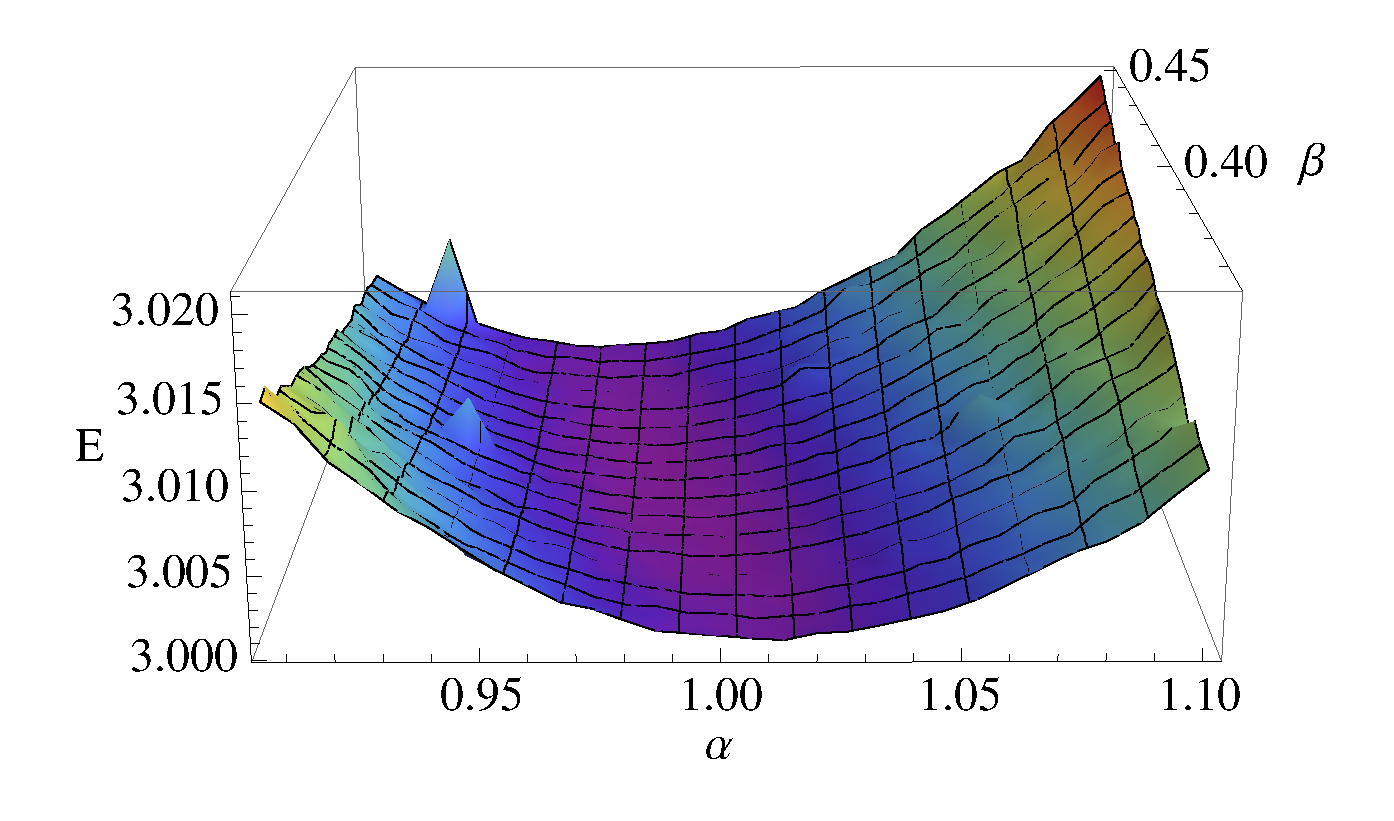
\includegraphics[scale=0.6]{2electron}
    \caption{Plot of $\alpha$- and $\beta$-dependencies of the ground state energy for two interacting electrons at the ground state.}
    \label{fig:2electron}
\end{figure}
\begin{figure}[htbp]
    \centering
    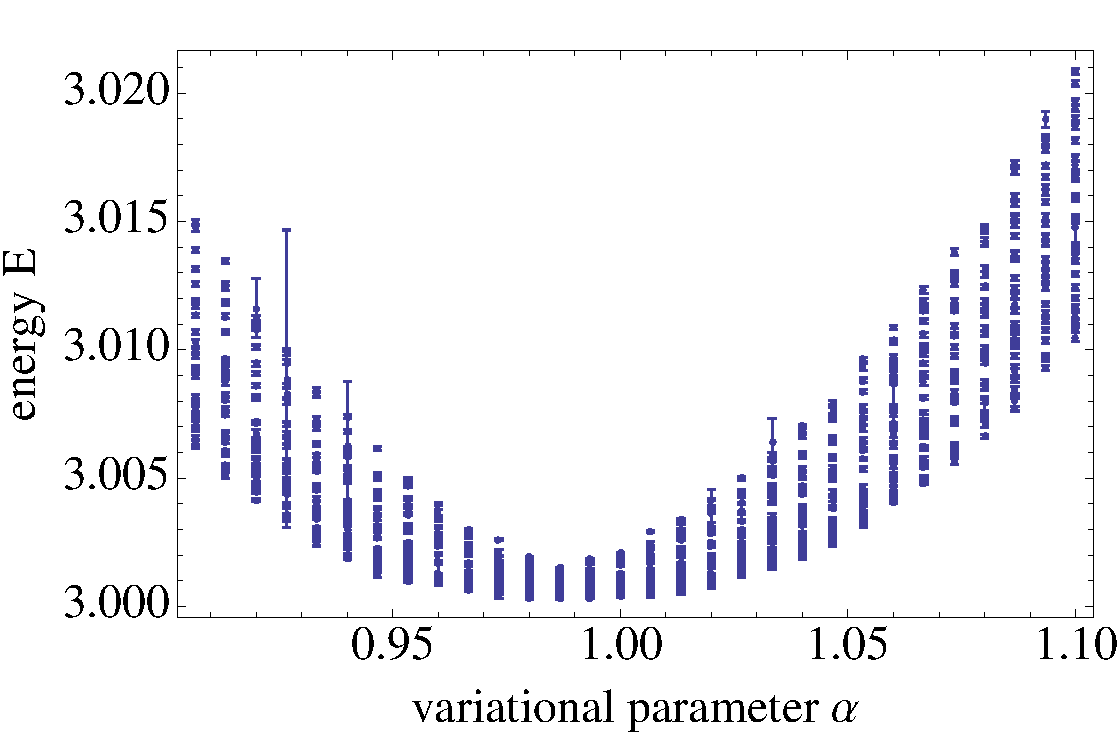
\includegraphics[scale=0.6]{2electronalpha}
    \caption{Plot of $\alpha$-dependency of the ground state energy for two interacting electrons at the ground state.}
    \label{fig:2electronalpha}
\end{figure}
\FloatBarrier
\subsubsection{Jastrow factor}
\subsubsection{Importance sampling: $\delta t$ dependency}
\subsection{Six electron case}
\subsubsection{Virial theorem}
\subsection{Analytical Calculations}\label{sec:analytical}